% Options for packages loaded elsewhere
\PassOptionsToPackage{unicode}{hyperref}
\PassOptionsToPackage{hyphens}{url}
%
\documentclass[
]{article}
\usepackage{lmodern}
\usepackage{amssymb,amsmath}
\usepackage{ifxetex,ifluatex}
\ifnum 0\ifxetex 1\fi\ifluatex 1\fi=0 % if pdftex
  \usepackage[T1]{fontenc}
  \usepackage[utf8]{inputenc}
  \usepackage{textcomp} % provide euro and other symbols
\else % if luatex or xetex
  \usepackage{unicode-math}
  \defaultfontfeatures{Scale=MatchLowercase}
  \defaultfontfeatures[\rmfamily]{Ligatures=TeX,Scale=1}
\fi
% Use upquote if available, for straight quotes in verbatim environments
\IfFileExists{upquote.sty}{\usepackage{upquote}}{}
\IfFileExists{microtype.sty}{% use microtype if available
  \usepackage[]{microtype}
  \UseMicrotypeSet[protrusion]{basicmath} % disable protrusion for tt fonts
}{}
\makeatletter
\@ifundefined{KOMAClassName}{% if non-KOMA class
  \IfFileExists{parskip.sty}{%
    \usepackage{parskip}
  }{% else
    \setlength{\parindent}{0pt}
    \setlength{\parskip}{6pt plus 2pt minus 1pt}}
}{% if KOMA class
  \KOMAoptions{parskip=half}}
\makeatother
\usepackage{xcolor}
\IfFileExists{xurl.sty}{\usepackage{xurl}}{} % add URL line breaks if available
\IfFileExists{bookmark.sty}{\usepackage{bookmark}}{\usepackage{hyperref}}
\hypersetup{
  pdftitle={Chaos in a Three-Species Food Chain},
  pdfauthor={Francis Banville, Élodie Basque and Gabriel Dansereau},
  hidelinks,
  pdfcreator={LaTeX via pandoc}}
\urlstyle{same} % disable monospaced font for URLs
\usepackage[left=3cm,right=3cm,top=2cm,bottom=2cm]{geometry}
\usepackage{longtable,booktabs}
% Correct order of tables after \paragraph or \subparagraph
\usepackage{etoolbox}
\makeatletter
\patchcmd\longtable{\par}{\if@noskipsec\mbox{}\fi\par}{}{}
\makeatother
% Allow footnotes in longtable head/foot
\IfFileExists{footnotehyper.sty}{\usepackage{footnotehyper}}{\usepackage{footnote}}
\makesavenoteenv{longtable}
\usepackage{graphicx,grffile}
\makeatletter
\def\maxwidth{\ifdim\Gin@nat@width>\linewidth\linewidth\else\Gin@nat@width\fi}
\def\maxheight{\ifdim\Gin@nat@height>\textheight\textheight\else\Gin@nat@height\fi}
\makeatother
% Scale images if necessary, so that they will not overflow the page
% margins by default, and it is still possible to overwrite the defaults
% using explicit options in \includegraphics[width, height, ...]{}
\setkeys{Gin}{width=\maxwidth,height=\maxheight,keepaspectratio}
% Set default figure placement to htbp
\makeatletter
\def\fps@figure{htbp}
\makeatother
\setlength{\emergencystretch}{3em} % prevent overfull lines
\providecommand{\tightlist}{%
  \setlength{\itemsep}{0pt}\setlength{\parskip}{0pt}}
\setcounter{secnumdepth}{-\maxdimen} % remove section numbering
\makeatletter
\@ifpackageloaded{subfig}{}{\usepackage{subfig}}
\@ifpackageloaded{caption}{}{\usepackage{caption}}
\captionsetup[subfloat]{margin=0.5em}
\AtBeginDocument{%
\renewcommand*\figurename{Figure}
\renewcommand*\tablename{Table}
}
\AtBeginDocument{%
\renewcommand*\listfigurename{List of Figures}
\renewcommand*\listtablename{\# List of tables}
}
\@ifpackageloaded{float}{}{\usepackage{float}}
\floatstyle{ruled}
\@ifundefined{c@chapter}{\newfloat{codelisting}{h}{lop}}{\newfloat{codelisting}{h}{lop}[chapter]}
\floatname{codelisting}{Listing}
\newcommand*\listoflistings{\listof{codelisting}{List of Listings}}
\makeatother
\usepackage[]{biblatex}
\addbibresource{bibliography.bib}

\title{Chaos in a Three-Species Food Chain}
\author{Francis Banville, Élodie Basque and Gabriel Dansereau}
\date{}

\begin{document}
\maketitle

\hypertarget{introduction}{%
\section{Introduction}\label{introduction}}

One of the main aspects of a biological community is its food web. The
first models of population dynamics generally considered the
interactions between only two species (e.g., \textcite{canale1970};
\textcite{rosenzweig1963}). However, in nature, food webs of two species
only influencing alone the behavior of the ecological network are quite
uncommon. Most of the time, they are way more complex and involve more
than two species (\textcite{hastings1991}). In that regard, some
researchers stated that every food webs study should involve at least
three species in order not to lose too much information
(\textcite{price1980}; \textcite{rosenzweig1973}).

At first, the principal interest of food webs researchers was related to
equilibrium analysis because they assumed that what was observed in
nature was the equilibrium state of dynamics models. Afterwards,
different studies declared that chaos played an important role in
ecological models. The simplest definition of chaos would be the extreme
sensibility of the system to its initial conditions in its resulting
behavior (\textcite{hastings1993}). This concept has been incorporated
in population dynamics during the mid-1970's. Since then, many papers
reinforced the importance of chaos in ecology.

\textcite{hastings1991}, who studied chaos in a continuous time model of
a food web including three species, contributed considerably to the
significance and understanding of this subject. Considering every aspect
of their model, their pioneer study led to a lot of other papers on food
webs dynamics and chaos (\textcite{brose2006}; \textcite{gakkhar2012}).
Replicating this kind of paper is important for many reasons. For
example, we can compare our results, obtained using current
technologies, with theirs and make available the code written to
recreate the model. In the current paper, we used the same equations and
parameters values as Hastings \& Powell to replicate their model. We
were able to reproduce all the figures in their paper using \emph{Julia
v1.1.0}.

\hypertarget{methods}{%
\section{Methods}\label{methods}}

The model formulation used in this paper is the same as the one in the
original publication. Hastings \& Powell used a 14 parameters model to
represent the three-species food chain, with \(X\), \(Y\), and \(Z\) as
the numbers of the species at the lowest level of the food chain, of the
species that preys upon \(X\), and of the species that preys upon \(Y\),
respectively. However, all of their analyses are based on a simpler
version of the model with nondimensional measures of time and population
sizes, hence 10 parameters only, with \(x\), \(y\) and \(z\) as the
standardized abundances of the three species. We chose to present this
simpler nondimensional version only in this paper, and we invite readers
to consult Hastings \& Powell's paper for more details on the original
dimensional parameters. Our model's formulation is given as:

\[ dx/dt = x(1 - x) - f_1(x)y \] \[ dy/dt = f_1(x)y - f_2(y)z - d_1y \]
\begin{equation} dz/dt = f_2(y)z - d_2z \label{eq:1}\end{equation}

with

\begin{equation} f_i(u) = a_iu/(1 + b_iu) \label{eq:2}\end{equation}

as the functional response.

The parameter values used in this paper are the same as the ones in the
original paper (Table~\ref{tbl:table1}). However, the initial conditions
of the simulations (i.e.~the values of \(x\), \(y\) and \(z\) at the
start) were not given in the original paper. This is an important
element to mention, as the initial conditions strongly affect the
simulations, particularly in the context of examining chaotic behavior.
We knew from figure 3 of the original paper that \(x \approx 0.75\), and
we tried to approximate \(y\) and \(z\) by trial and errors. In order to
replicate the original figures as closely as possible, we used different
initial conditions in all of our representations to present the closest
matching graphical result. The conditions used are specified in each
figure. We believe that the use of such different conditions do not
alter the results' interpretation.

\hypertarget{tbl:table1}{}
\begin{longtable}[]{@{}ll@{}}
\caption{\label{tbl:table1}Nondimensional parameters and the values used
in the simulations}\tabularnewline
\toprule
Nondimensional parameters & Values\tabularnewline
\midrule
\endfirsthead
\toprule
Nondimensional parameters & Values\tabularnewline
\midrule
\endhead
\(a_1\) & 5.0\tabularnewline
\(b_1\) & varied from 2.0 to 6.2\tabularnewline
\(a_2\) & 0.1\tabularnewline
\(b_2\) & 2.0\tabularnewline
\(d_1\) & 0.4\tabularnewline
\(d_2\) & 0.01\tabularnewline
\bottomrule
\end{longtable}

As noted by Hastings \& Powell, numerical integration is the only way to
investigate the global dynamical behavior of the system. We used
\emph{Julia version 1.1.0} (\textcite{bezanson2017}), along with
packages ``DifferentialEquations.jl'' to compute the numerical
integrations, ``ParameterizedFunctions.jl'' to simplify the
parameterized function call, and ``Plot.jl'' to represent our results.
We let the \texttt{solve} function select the appropriate algorithm to
solve our differential equations, as we believe such a function to be
more precise at determining the correct algorithm. In our
implementation, it selected a composite algorithm combining, amongst
others, algorithms Tsit5 and Rosenbrock23.

In order to replicate figure 2 of the original paper, we followed
Hastings \& Powell's method and let our system run for 10 000 time
steps. We then represented the system's behavior by plotting the species
nondimensional variables against time (between time steps 5000 and 6500,
which eliminates transient behavior), as well as a three dimensional
phase plot of the three species (for all time steps). Note that in the
case of the three dimensional phase plot, we had to set RK4 as the
solving algorithm, as well as a relative tolerance of \(1e-14\); if not,
the representation was unexpectedly different from the original paper.
In order to illustrate the dynamics of the model, we created a Graphics
Interchange Format (GIF) file of the three-dimensional phase plot that
showed the trajectories of \(x\), \(y\) and \(z\) for the selected
parameters (in supplement of this paper).

To replicate figure 3 and illustrate the effect of a small change in
initial conditions, we plotted the trajectory for species \(x\) between
time steps 0 and 500 starting at \(x\) = 0.77, then changed the initial
\(x\) value by 0.01 (to \(x\) =0.78) and plotted the new trajectory for
the same interval on the same graph.

To replicate figure 4, we constructed a bifurcation diagram for species
\(z\) where we varied values of \(b_1\) from 2.2 to 6.2 in steps of
0.01. However, our approach had to be slightly different. Hastings \&
Powell constructed what we consider a special type of bifurcation
diagram, representing only the maxima of \(z\) as a function of \(b_1\),
rather than all possible values in the system's behavior, as in a
typical logistic bifurcation diagram for example. This raised the
problem of correctly identifying the maxima values in the cycling
dynamic. Moreover, Hastings \& Powell mentioned that, in order to
clarify their figure, they eliminated points resulting from the
appearance of secondary local maxima in the cycling dynamics of species
\(z\), but they did not provide details on how they identified such
points. Hence, we adopted the following method: 1) we selected the 1000
last solutions for our system between time steps 1 and 10 000, in order
to eliminate transient behavior; 2) we selected the values that were
greater than both their preceding and following values, which identified
local maxima only; and 3) we only kept values that were greater than a
given threshold of the cycle's maximal amplitude, in order to remove
secondary local maxima. We determined by trial and errors that the best
threshold was 66\%, as it best removed values in apparent second
branches of \(b_1\) while keeping the values in the primary branch. We
note however that for some values of \(b_1\), the true solutions of the
system were unstable and that the system did not reach a cycling
behavior within 10 000 steps. For these values of \(b_1\) (37 values,
all between 5.01 and 6.2), we could not present any values of \(z\) in
our bifurcation diagram.

Hastings \& Powell mentioned in their original paper that they also
examined the system's behavior when varying \(b_2\) instead of \(b_1\),
although they did not present the results. We examined the same behavior
by constructing another bifurcation diagram of \(z\) for values of
\(b_2\) varying from 1.5 to 3.2, using the same method as described
above. We fixed \(b_1 = 3.0\), as it is the example used to illustrate
chaotic behavior throughout Hastings \& Powell's paper.

In order to replicate Hastings \& Powell's figure 5, we solved the
system of differential equations using the abovementioned algorithm RK4,
as well as a relative tolerance of \(1e-14\). We used \(b_1 = 3.0\) and
\(b_1 = 6.0\), as in the original paper, to replicate its subfigures a-b
and c-d, respectively. We defined planes of equation \(z = 9.0\) and
\(z = 3.0\) for those subfigures, respectively, as these intercepted the
``handles'' of their respective three-dimensional phase plot. We defined
those ``handles'' as in Hastings \& Powell, that is as the region in the
phase plots where z declines from its maxima to its minima. However, we
had to use a tolerance value \(epsilon\) of 0.05 in order to identify
the points whose distance from the plane was negligible (i.e.~their
\(z\) values ranging between 8.95-9.05 and 2.95-3.05, respectively),
since we were not able to find the phase plots' exact interception
points. We specified the planes' \(x\) and \(y\) coordinates to retain
only the points that were in the ``handles'' (subfigures (a-b): \(x\)
and \(y\) ranging between 0.95-0.98 and 0.015-0.040, respectively;
subfigures (c-d): \(x\) and \(y\) ranging between 0.93-1.00 and
0.00-0.09, respectively). As in the original paper, we recreated the
Poincaré sections (subfigures (a) and (c)), by plotting \(y\) against
\(x\) coordinates of the retained points, and the Poincaré maps
(subfigures (b) and (d)), by plotting \(x\) coordinates of the retained
points (\(x(n)\)) against that of their immediate subsequent retained
points (\(x(n+1)\)). Since Hastings and Powell's figure 5 (e) only
schematized the plane in the three-dimensional phase plot, we did not
reproduce it.

The objective of this paper being to reproduce the main results of the
original paper, we did not reproduce its figure 1, which was only a
schematic representation of the three-species food chain. All the code
used to replicate the original paper is available alongside the article.

\hypertarget{results}{%
\section{Results}\label{results}}

We were able to replicate Hastings \& Powell's main findings, even
without knowing their exact algorithm and sets of initial conditions.
First, our time series of the nondimensional variables
(Fig.~\ref{fig:fig2}) present similar patterns as those identified by
Hastings and Powell. We observed that the standardized population
densities of \(x\), \(y\), and \(z\) (Eq.~\ref{eq:1}, Eq.~\ref{eq:2})
oscillate in a period of around 125 time steps. Within a cycle, the
population densities of species \(x\) and \(y\) oscillate while that of
species \(z\) grows until it reaches its primary local maximum (see
definition in methods), at which \(y\) and \(x\) respectively reach
their local minimum and maximum values. \(z\) then declines until it
reaches its local minimum, forming the ``handle'' of the teacup
(Fig.~\ref{fig:fig2d}), and subsequently beginning a new cycle. The
animated figure we produced illustrates this dynamic (see supp. online
material). Although slight discrepancies exist between our results and
those of Hastings \& Powell, they did not seem to strongly influence the
abovementioned period length, nor the values of the local maxima and
minima of the dimensionless variables. Indeed, \(x\) varies
approximately from 0.2 to 1.0, \(y\) from 0.0 to 0.4, and \(z\) from 7.5
to 10.5 (Fig.~\ref{fig:fig2}), as seen in the original paper.

Second, the time series of \(x\) from \(t = 0\) to \(500\) supports the
chaotic behavior of the system, with slightly different initial
conditions leading to increasingly different
trajectories(Fig.~\ref{fig:fig3}). The values themselves are almost
identical to Hastings \& Powell's until \(t \approx 250\), at which
point they start to diverge, but this behavior was to be expected
without the exact same initial conditions.

Third, our bifurcation diagrams (Fig.~\ref{fig:fig4}) have the same
general shapes as the ones of Hastings \& Powell, and are in the same
range of \(z_{max}\). We identified most of the local maxima of \(z\)
found in the original paper for \(b_1\) ranging from 2.2 to 6.2.
However, we missed some of them and we found others that were absent in
their paper. For instance, for \(b_1\) = 3.1, we found multiple local
maxima of \(z\), whereas Hastings \& Powell had only found a dichotomy
of values. The differences are even more apparent in Fig.~\ref{fig:fig4}
(c), which represents a detailed portion of Fig.~\ref{fig:fig4} (a). For
example, contrary to their findings, we did identify local maxima values
for \(b_1\) ranging from 2.30 and 2.35. In other words, we did not
observe the significant gap in the bifurcation diagram that they had
found.

Our additional bifurcation diagrams, where we varied \(b_2\) instead of
\(b_1\) (Fig.~\ref{fig:figS1}), confirm that chaos occurs for values
other than \(b_2\) = 2.0. Chaos is apparent for both smaller or greater
values. However, while Hastings \& Powell reported that chaos was more
likely for greater values of \(b_2\), our results highlight that \(z\)
instead converges to a single value and starts to crash past \(b_2\) =
2.35.

Lastly, although Hastings and Powell did not specify the equation of the
plane that crosses the trajectories of the phase plot at its ``handle'',
we were able to accurately replicate their Poincaré section and map for
\(b_1\) = 3.0 (Fig.~\ref{fig:fig5} (a, b)). The main discordance lies in
the number of points that cross the plane, and consequently on the
apparent smoothness of the graphs. On the contrary, it was harder to
precisely replicate the Poincaré map for \(b_1\) = 6.0
(Fig.~\ref{fig:fig5} (d)), even though the corresponding reproduced
Poincaré section (Fig.~\ref{fig:fig5} (c)) was similar to the one in
Hastings \& Powell's paper.

\hypertarget{discussion}{%
\section{Discussion}\label{discussion}}

We were able to replicate the chaotic behaviour displayed by Hastings \&
Powell's model. The resulting behavior is indeed very sensible to the
initial conditions, showing increasingly diverging trajectories
(Fig.~\ref{fig:fig3}) for slightly different parameters, as well as
unending oscillations (Fig.~\ref{fig:fig2}). The bifurcation diagrams
(Fig.~\ref{fig:fig4}) further confirm the existence of chaos by
illustrating the presence of cyclic behavior for some values and chaotic
intervals for others, hence the extreme sensibility of the system to
\(b_1\) values. As for the Poincaré sections (Fig.~\ref{fig:fig5} (a,
c)), Hastings \& Powell plotted (x,y) coordinates of points of the phase
plots that theoretically coincided with the plane in the ``handle'' of
the teacup-shaped diagrams. The Poincaré sections being almost
unidimensional, we considered, as explained in the original paper, a
single variable within our Poincaré maps (Fig.~\ref{fig:fig5} (b, d)).
The slopes of these latter graphs therefore also denoted chaos, as
specified by Hastings \& Powell.

For Fig.~\ref{fig:fig2} and Fig.~\ref{fig:fig3}, the shape of the cycles
and oscillations are similar to Hastings and Powell's. As mentioned
earlier, the slight differences are due to the fact that we surely did
not use the exact same initial conditions as the original authors. Such
difference is to be expected with a system exhibiting chaotic behavior
and do not alter the results interpretation.

The difference between our Fig.~\ref{fig:fig4} and Hastings \& Powell's
bifurcation diagram is more intriguing. Admittedly, we could not figure
out exactly what Hastings \& Powell's method was, and some elements such
as identifying maxima values by increasing \(b_1\) first, then by
decreasing it, did not make sense to us. Our method should be
appropriate, theoretically, to select only values that are primary local
maxima, and it did seem to work very well for most \(b_2\) values; yet,
the broad range of values that we observed at \(b_1\) = 3.1 instead of a
dichotomy is hard to explain. It seems unlikely that the problem could
be related to our arbitrary threshold of 66\% or to our identification
of a local maximum, because we would then be either missing some lower
values or having too many, not having more in between. The timeseries of
all values of \(z\) (not presented here) for \(b_1\) = 3.1 confirms that
there are ``intermediate'' maxima values, which should be selected by
any proper method. We suggest that the difference might be due to the
algorithms used for the numerical integration in our two studies. It is
possible that the relationship between the parameters at this point is
such that a small difference in algorithm might have an important
impact. It is also possible that their algorithm came up with an
unstable solution and a system that did not reach cycling behavior, such
as ours for certain values past \(b_1\) = 5.01, but that Hastings \&
Powell's method selected some values anyways, explaining the behavior at
\(b_1\) = 3.1.

While we also found chaos for values of \(b_2\) other than the default
one of 2.0, both smaller or greater, we do not totally agree with
Hastings \& Powell that ``chaos is more likely for larger values of
\(b_2\)''. As Fig.~\ref{fig:figS1}, chaos can be quite likely for both
smaller or larger values. We find important to note, however, that at a
certain value of \(b_2\), \(z\) converges and starts to crash, thus
exhibiting non chaotic behavior within a given range of \(b_1\) values.
This crash is to be expected when looking at the original dimensional
parameters, so it is possible that Hastings \& Powell simply chose not
to reach this limit in their analyses, as they were only interested in
biologically reasonable parameters likely to occur with the three
species present.

We believe that our mixed results in attempting to replicate
Fig.~\ref{fig:fig5} came from the algorithm we used to identify the
points that coincided with the plane. For instance, we had to specify a
tolerance value (\(epsilon\)), which defined a region under and above
the plane. Although we were able to precisely replicate the Poincaré
sections for \(b_1\) = 3.0 (Fig.~\ref{fig:fig5} (a)) and 6.0
(Fig.~\ref{fig:fig5} (c)), the Poincaré maps need some refinement. For
\(b_1\) = 3.0 (Fig.~\ref{fig:fig5} (b)), it lacked some points of the
phase plots and included others that were closed yet non-coincident with
the plane. For \(b_1\) = 6.0 (Fig.~\ref{fig:fig5} (d)), the discrepancy
was more obvious, and might be due to the more chaotic behavior of the
system under this parameter, observed for example from the larger width
of its ``handle'' (compare axis intervals of Fig.~\ref{fig:fig5} (a,
c)). We are still working on improving our algorithms to adequately
replicate Hastings \& Powell's Poincaré maps.

We have succeeded in replicating Hastings \& Powell's model and its main
findings, as our results confirm chaos arising in a three species food
chain in continuous time. In general, the model, including its equations
and parameters, was well described by the authors. The most significant
flaws of Hastings \& Powell's paper in terms of replication were the
absence of the values of the initial conditions, which have a huge
impact on a chaotic system, and the insufficient description of certain
methods. Consequently, there are slight differences between our results
and theirs. Furthermore, since we tried to keep our implementation as
close as possible to the original one, some steps did rely on arbitrary
thresholds (for instance for the primary local maxima or the Poincaré
sections and maps boundaries). Hence, our replication is somewhat not
very flexible and possibly could not be applied to a broader range of
parameter values. We suggest that an interesting step forward would be
to train machine-learning algorithms, such as neural networks, to
identify chaotic behavior and its boundaries, in order to obtain an even
better performing implementation.

\begin{figure}
\hypertarget{fig:fig2}{%
\centering
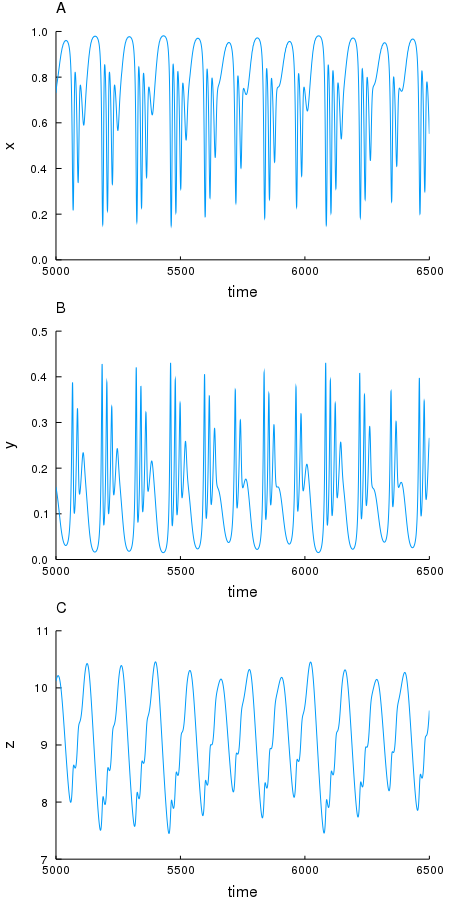
\includegraphics{figures/fig2.png}
\caption{Time series of the nondimensional variables (a) \(x\), (b)
\(y\) and (c) \(z\), for \(t\) ranging from 5000 to 6500 (\(x\) = 1.0,
\(y\) = 1.0, and \(z\) = 1.0 as initial conditions). The parameter
values used in the simulations are given in Table~\ref{tbl:table1}
(\(b_1\) = 3.0). This figure replicates fig.~2 (a-b-c) of Hastings \&
Powell.}\label{fig:fig2}
}
\end{figure}

\begin{figure}
\hypertarget{fig:fig2d}{%
\centering
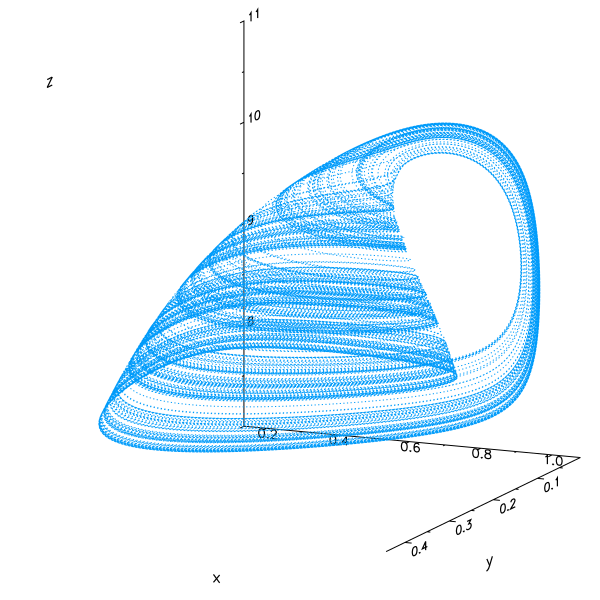
\includegraphics{figures/fig2d.png}
\caption{Three-dimensional phase plot of species \(x\), \(y\) and \(z\)
for \(t\) ranging from 1 to 10 000 (\(x\) = 0.7, \(y\) = 0.2, and \(z\)
= 8.0 as initial conditions). The parameter values used in the
simulations are given in Table~\ref{tbl:table1} (\(b_1\) = 3.0). This
figure replicates fig.~2 (d) of Hastings \& Powell.}\label{fig:fig2d}
}
\end{figure}

\begin{figure}
\hypertarget{fig:fig3}{%
\centering
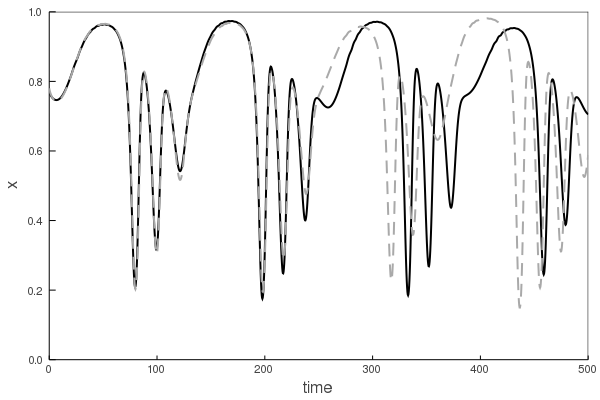
\includegraphics{figures/fig3.png}
\caption{Time series of \(x\), for \(t\) ranging from 0 to 500. The
solid and dash lines have \(x\) = 0.77 and \(x\) = 0.78 as initial
conditions respectively (\(y\) = 0.16 and \(z\) = 9.9 as initial
conditions are unchanged). The parameter values used in the simulations
are given in Table~\ref{tbl:table1} (\(b_1\) = 3.0). This figure
replicates fig.~3 of Hastings \& Powell.}\label{fig:fig3}
}
\end{figure}

\begin{figure}
\hypertarget{fig:fig4}{%
\centering
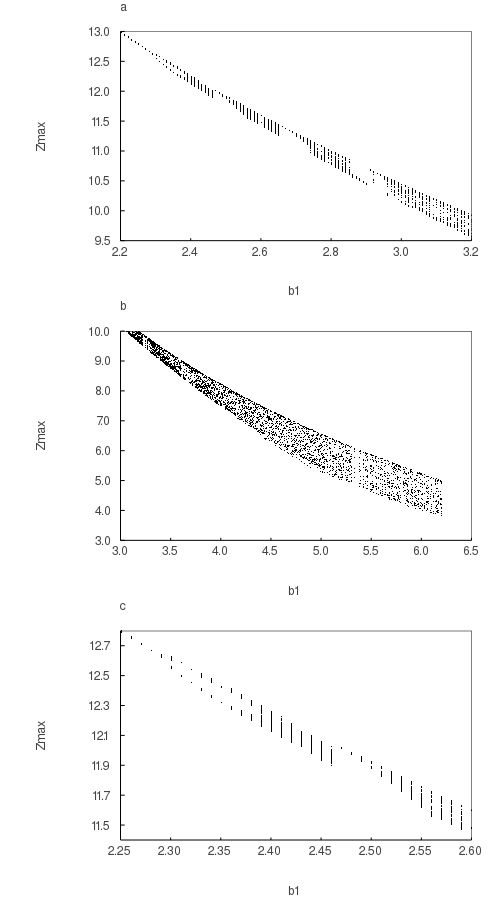
\includegraphics{figures/fig4.png}
\caption{Bifurcation diagrams of the local maxima of \(z\) plotted
against \(b_1\) ranging from (a) 2.2 to 3.2, (b) 3.0 to 6.2, and (c)
2.25 to 2.6. The other parameter values used in the simulations are
given in Table~\ref{tbl:table1} (\(x\) = 1.0, \(y\) = 1.0, and \(z\) =
1.0 as initial conditions). This figure replicates fig.~4 of Hastings \&
Powell.}\label{fig:fig4}
}
\end{figure}

\begin{figure}
\hypertarget{fig:fig5}{%
\centering
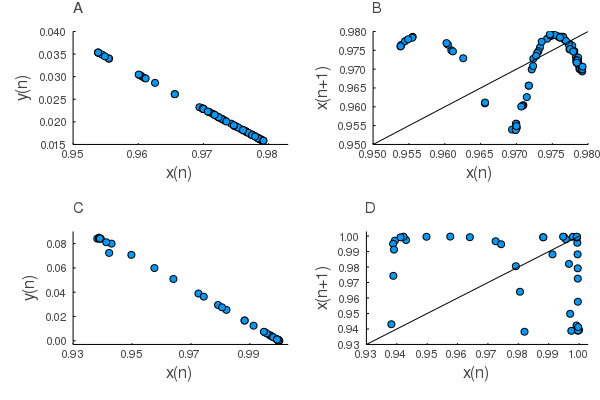
\includegraphics{figures/fig5.png}
\caption{(a) and (b) Poincaré section and map, respectively, for the
parameter values given in Table~\ref{tbl:table1} (\(b_1\) = 3.0). (c)
and (d) Poincaré section and map for the same parameter values except
\(b_1\) = 6.0. All sets of initial values are unchanged (\(x\) = 0.7,
\(y\) = 0.2, \(z\) = 8.0). The solid lines of equation \(x(n+1) = x(n)\)
are shown in (b) and (d). This figure replicates fig.~5 of Hastings \&
Powell, except their fig.~5 (e), which is partly reproduced in our
fig.~2 (d).}\label{fig:fig5}
}
\end{figure}

\begin{figure}
\hypertarget{fig:figS1}{%
\centering
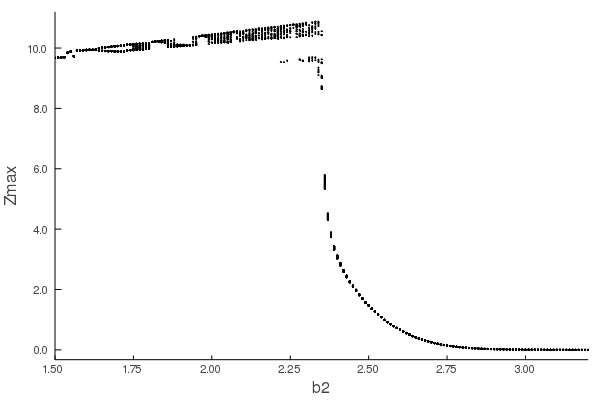
\includegraphics{figures/figS1.png}
\caption{Bifurcation diagrams of the local maxima of \(z\) plotted
against \(b_2\) ranging from 1.5 to 3.2. The other parameter values used
in the simulations are given in Table~\ref{tbl:table1} (\(x\) = 1.0,
\(y\) = 1.0, and \(z\) = 1.0 as initial conditions, \(b_1\) =
3.0).}\label{fig:figS1}
}
\end{figure}

\printbibliography

\end{document}
